% !TEX TS-program = lualatex
% !TEX encoding = UTF-8 Unicode
\documentclass{article}
\usepackage{lmodern}
\usepackage{graphicx}
\graphicspath{{doc/assets/}{../doc/assets/}{assets/}{../assets/}{../}}

\usepackage[
  paperwidth=338mm, paperheight=190mm,
  top=0mm, bottom=0mm, left=0mm, right=0mm
]{geometry}

% -- ROBUST FONT FIX FOR LUALATEX & OVERLEAF --
\usepackage{fontspec}
\IfFontExistsTF{Roboto}{
  \setsansfont{Roboto}
}{
  \IfFontExistsTF{Arial}{
    \setsansfont{Arial}[
      ItalicFont={Arial},
      ItalicFeatures={FakeSlant=0.25},
      BoldFont={Arial Bold},
      BoldItalicFont={Arial Bold},
      BoldItalicFeatures={FakeSlant=0.25}
    ]
  }{
    \IfFontExistsTF{Noto Sans}{
      \setsansfont{Noto Sans}
    }{
      \IfFontExistsTF{Liberation Sans}{
        \setsansfont{Liberation Sans}
      }{
        \IfFontExistsTF{TeX Gyre Heros}{
          \setsansfont{TeX Gyre Heros}
        }{
          % Fallback mặc định
        }
      }
    }
  }
}
\renewcommand{\familydefault}{\sfdefault}
% ---------------------------------------------

\usepackage{xcolor}
\usepackage{tikz}
\usepackage{fontawesome5}
\usepackage[hidelinks]{hyperref}
\pagestyle{empty}
\parindent=0pt

%── Bảng màu chuẩn hóa thanh lịch (Sửa lỗi thiếu định nghĩa cbk)
\definecolor{sap}{HTML}{0000FF}           % Primary: Xanh lam thuần
\definecolor{cyel}{HTML}{FFFF00}         % Secondary: Vàng thuần
\definecolor{cslate}{HTML}{64748B}
\definecolor{cneg}{HTML}{D32F2F}
\definecolor{cpos}{HTML}{2E7D32}
\definecolor{cgry}{HTML}{757575}
\definecolor{clightgray}{HTML}{F8F9FA}
\definecolor{cbk}{HTML}{424242}          % Sửa lỗi: Khai báo màu cbk cho text nội dung

\newcommand{\TitleLine}[1]{%
  \draw[cyel, line width=6pt] (17mm, -10mm) -- (17mm, -25mm);
  \node[anchor=west, font=\fontsize{35}{40}\selectfont\bfseries, text=sap] at (21mm, -17.5mm) {#1};
}

\begin{document}

% ===================================================================
% SLIDE 13: Nguồn gốc xung đột
% ===================================================================
\begin{tikzpicture}[remember picture, overlay]
  \coordinate (NW) at (current page.north west);
  \begin{scope}[shift={(NW)}]
    \TitleLine{Nguồn gốc xung đột}

    % Column 1: Developer vs Tester
    \begin{scope}[shift={(17mm, -50mm)}]
        \node[anchor=north, font=\fontsize{22}{26}\selectfont\bfseries\color{sap}, text width=95mm, align=center] at (47.5mm, 0) {
            \faLaptopCode\ \ \normalsize{vs}\ \ \Large{\faVial} \\
            \vspace{8pt}
            \fontsize{14}{18}\selectfont\color{cbk} Lập trình viên \& Kiểm thử viên
        };
        \node[anchor=north] at (47.5mm, -25mm) {
            
\includegraphics[width=90mm, height=100mm, keepaspectratio]{slide_testerVsDeveloper.jpg}
        };
    \end{scope}

    % Column 2: Overleaf vs VSCode (GitHub)
    \begin{scope}[shift={(120mm, -50mm)}]
        \node[anchor=north, font=\fontsize{22}{26}\selectfont\bfseries\color{sap}, text width=95mm, align=center] at (47.5mm, 0) {
            \faLeaf\ \ \normalsize{vs}\ \ \Large{\faCode} \\
            \vspace{8pt}
            \fontsize{14}{18}\selectfont\color{cbk} Overleaf \& Nền tảng Git
        };
        \node[anchor=north] at (47.5mm, -25mm) {
            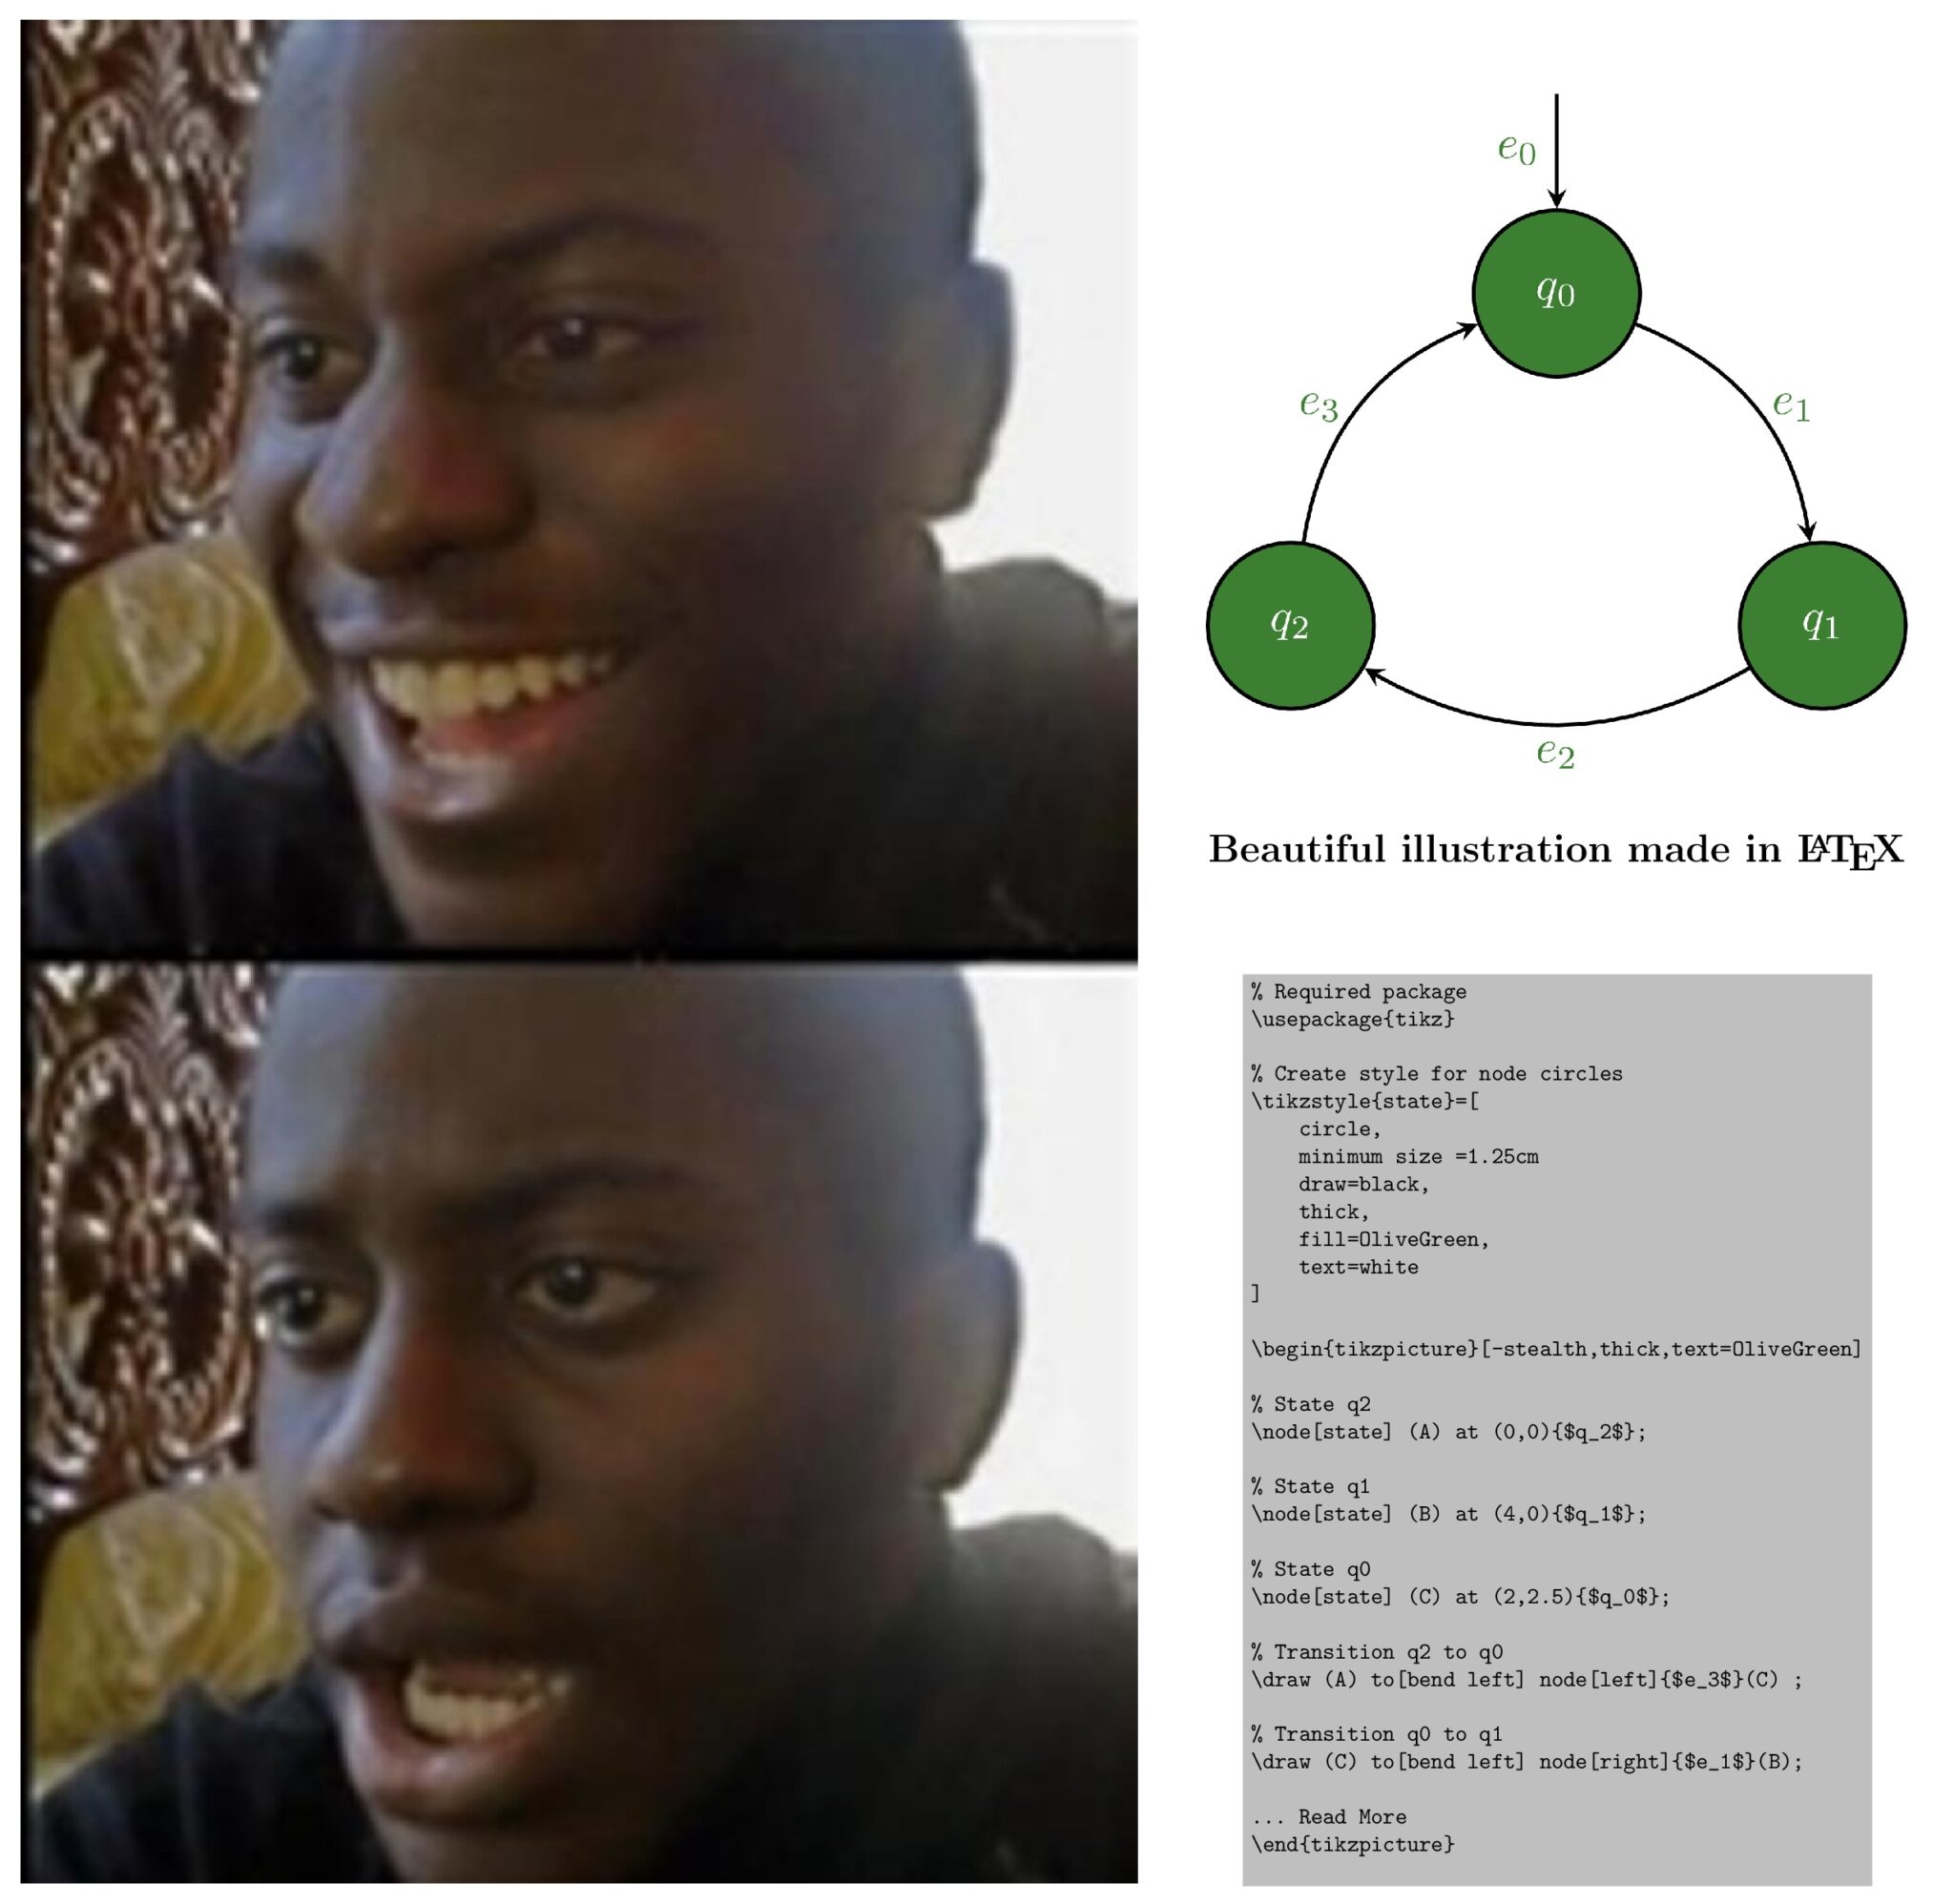
\includegraphics[width=90mm, height=100mm, keepaspectratio]{slide_latexMeme.jpg}
        };
    \end{scope}

    % Column 3: Desktop vs Mobile
    \begin{scope}[shift={(223mm, -50mm)}]
        \node[anchor=north, font=\fontsize{22}{26}\selectfont\bfseries\color{sap}, text width=95mm, align=center] at (47.5mm, 0) {
            \faDesktop\ \ \normalsize{vs}\ \ \Large{\faMobile} \\
            \vspace{8pt}
            \fontsize{14}{18}\selectfont\color{cbk} Desktop \& Web (WASM)
        };
        \node[anchor=north] at (47.5mm, -25mm) {
            
\includegraphics[width=90mm, height=100mm, keepaspectratio]{slide_crossPlatformMeme.png}
        };
    \end{scope}

  \end{scope}
\end{tikzpicture}
\newpage

% ===================================================================
% SLIDE 14: Giải quyết xung đột
% ===================================================================
\begin{tikzpicture}[remember picture, overlay]
  \coordinate (NW) at (current page.north west);
  \begin{scope}[shift={(NW)}]
    \TitleLine{Giải quyết xung đột}

    % Column 1: Branching Strategy
    \begin{scope}[shift={(17mm, -50mm)}]
        \fill[clightgray, rounded corners=4pt] (0,0) rectangle (95mm, -100mm);
        \node[anchor=north west, font=\fontsize{18}{22}\selectfont\bfseries\color{sap}, text width=85mm] at (5mm, -10mm) {
            \faCodeBranch\ \ Chiến lược rẽ nhánh
        };
        \node[anchor=north west, font=\fontsize{14}{20}\selectfont\color{cbk}, text width=85mm, align=left] at (5mm, -30mm) {
            Áp dụng chiến lược phân chia module và rẽ nhánh (branching) độc lập.
            Giúp cô lập tính năng và hạn chế rủi ro dẫm chân lên nhau khi lập trình song song.
        };
    \end{scope}

    % Column 2: GitHub -> Slack
    \begin{scope}[shift={(120mm, -50mm)}]
        \fill[clightgray, rounded corners=4pt] (0,0) rectangle (95mm, -100mm);
        \node[anchor=north west, font=\fontsize{18}{22}\selectfont\bfseries\color{sap}, text width=85mm] at (5mm, -10mm) {
            \faGithub\ \ Tích hợp GitHub
        };
        \node[anchor=north west, font=\fontsize{14}{20}\selectfont\color{cbk}, text width=85mm, align=left] at (5mm, -30mm) {
            Tích hợp cảnh báo từ GitHub trực tiếp vào không gian Slack.
            Đảm bảo luồng giao tiếp liên tục để kịp thời xử lý các xung đột mã nguồn.
        };
    \end{scope}

    % Column 3: Trello -> Slack
    \begin{scope}[shift={(223mm, -50mm)}]
        \fill[clightgray, rounded corners=4pt] (0,0) rectangle (95mm, -100mm);
        \node[anchor=north west, font=\fontsize{18}{22}\selectfont\bfseries\color{sap}, text width=85mm] at (5mm, -10mm) {
            \faTrello\ \ Đồng bộ Trello
        };
        \node[anchor=north west, font=\fontsize{14}{20}\selectfont\color{cbk}, text width=85mm, align=left] at (5mm, -30mm) {
            Thiết lập liên kết tự động đẩy thông báo từ Trello về Slack.
            Giúp toàn đội nắm bắt tiến độ dự án theo thời gian thực một cách liền mạch.
        };
    \end{scope}

  \end{scope}
\end{tikzpicture}
\newpage

% ===================================================================
% SLIDE 15: Bài học làm việc nhóm
% ===================================================================
\begin{tikzpicture}[remember picture, overlay]
  \coordinate (NW) at (current page.north west);
  \begin{scope}[shift={(NW)}]
    \TitleLine{Bài học làm việc nhóm}

    % Layer 1: Single File Development
    \begin{scope}[shift={(17mm, -45mm)}]
        \fill[clightgray, rounded corners=4pt] (0,0) rectangle (304mm, -40mm);
        \fill[sap, rounded corners=4pt] (0,0) rectangle (40mm, -40mm);
        \node[text=white, font=\fontsize{35}{40}\selectfont] at (20mm, -20mm) {\faFileCode};
        \node[anchor=north west, font=\fontsize{18}{22}\selectfont\bfseries\color{sap}] at (48mm, -6mm) {Kỷ luật mã nguồn trong tệp đơn (Single File)};
        \node[anchor=north west, font=\fontsize{14}{19}\selectfont\color{cbk}, text width=245mm, align=left] at (48mm, -16mm) {
            Khi phát triển trên một tệp mã nguồn duy nhất, cấu trúc sạch là yếu tố sống còn.
            Đội ngũ nhận ra sự cần thiết của việc phân chia các khối logic rõ ràng và tuân thủ nguyên tắc viết chú thích (comment) chi tiết bằng tiếng Việt để hỗ trợ việc tra cứu và tiếp quản chéo dễ dàng hơn.
        };
    \end{scope}

    % Layer 2: Learn Git
    \begin{scope}[shift={(17mm, -95mm)}]
        \fill[clightgray, rounded corners=4pt] (0,0) rectangle (304mm, -40mm);
        \fill[sap, rounded corners=4pt] (0,0) rectangle (40mm, -40mm);
        \node[text=white, font=\fontsize{35}{40}\selectfont] at (20mm, -20mm) {\faGit};
        \node[anchor=north west, font=\fontsize{18}{22}\selectfont\bfseries\color{sap}] at (48mm, -6mm) {Trang bị nền tảng Git trước khi làm việc nhóm};
        \node[anchor=north west, font=\fontsize{14}{19}\selectfont\color{cbk}, text width=245mm, align=left] at (48mm, -16mm) {
            Quản lý mã nguồn không chỉ là lưu trữ mà là sự phối hợp.
            Toàn bộ thành viên cần làm chủ các thao tác Git cơ bản, luồng rẽ nhánh và cách giải quyết xung đột (conflict) trước khi code chung.
            Điều này giúp ngăn chặn triệt để rủi ro ghi đè mã nguồn và tiết kiệm thời gian gỡ lỗi.
        };
    \end{scope}

    % Layer 3: Design First
    \begin{scope}[shift={(17mm, -145mm)}]
        \fill[clightgray, rounded corners=4pt] (0,0) rectangle (304mm, -40mm);
        \fill[sap, rounded corners=4pt] (0,0) rectangle (40mm, -40mm);
        \node[text=white, font=\fontsize{35}{40}\selectfont] at (20mm, -20mm) {\faPencilRuler};
        \node[anchor=north west, font=\fontsize{18}{22}\selectfont\bfseries\color{sap}] at (48mm, -6mm) {Tư duy thiết kế đi trước (Design First, Code Later)};
        \node[anchor=north west, font=\fontsize{14}{19}\selectfont\color{cbk}, text width=245mm, align=left] at (48mm, -16mm) {
            \textit{"Think about design first before coding"}.
            Bài học đắt giá nhất là không vội viết mã khi chưa thống nhất kiến trúc tổng thể.
            Phác thảo sơ đồ, định nghĩa cấu trúc dữ liệu và luồng hệ thống từ những ngày đầu giúp nền tảng vững chắc, hạn chế tối đa rủi ro đập đi xây lại.
        };
    \end{scope}

  \end{scope}
\end{tikzpicture}
\newpage

\end{document}